\documentclass[a4paper]{article}

\usepackage{INTERSPEECH2021}
\usepackage{cite}
\usepackage{booktabs}
\usepackage{hyperref}
\usepackage[noabbrev,capitalize]{cleveref}

\hypersetup{
    colorlinks=true,
    linkcolor=black,
    filecolor=black,      
    citecolor=black,
    urlcolor=black,
    pdfpagemode=FullScreen,
}

% https://tex.stackexchange.com/questions/83085/how-to-improve-listings-display-of-json-files
\usepackage{bera}% optional: just to have a nice mono-spaced font
\usepackage{listings}
\usepackage{xcolor}

\colorlet{punct}{red!60!black}
\definecolor{background}{HTML}{EEEEEE}
\definecolor{delim}{RGB}{20,105,176}
\colorlet{numb}{magenta!60!black}

\lstdefinelanguage{json}{
    basicstyle=\normalfont\ttfamily,
    numbers=left,
    numberstyle=\scriptsize,
    stepnumber=1,
    numbersep=8pt,
    showstringspaces=false,
    breaklines=true,
    frame=lines,
    backgroundcolor=\color{background},
    literate=
     *{0}{{{\color{numb}0}}}{1}
      {1}{{{\color{numb}1}}}{1}
      {2}{{{\color{numb}2}}}{1}
      {3}{{{\color{numb}3}}}{1}
      {4}{{{\color{numb}4}}}{1}
      {5}{{{\color{numb}5}}}{1}
      {6}{{{\color{numb}6}}}{1}
      {7}{{{\color{numb}7}}}{1}
      {8}{{{\color{numb}8}}}{1}
      {9}{{{\color{numb}9}}}{1}
      {:}{{{\color{punct}{:}}}}{1}
      {,}{{{\color{punct}{,}}}}{1}
      {\{}{{{\color{delim}{\{}}}}{1}
      {\}}{{{\color{delim}{\}}}}}{1}
      {[}{{{\color{delim}{[}}}}{1}
      {]}{{{\color{delim}{]}}}}{1},
}

\title{Final NLU project}
\name{Francesco Bozzo (mat. 229312)}

\address{
  University of Trento}
\email{francesco.bozzo@studenti.unitn.it}

\begin{document}

\maketitle

% Dear students, \\
% here you can find a complete description of the sections that are mandatory for your project and you need to address them during the development, as well as your 4-page (+1 for References) project report.


\section{Introduction}
% brief summary of what you have done (approx. 100 words)
This project presents some deep learning techniques to predict intents and slots in a multitask learning setting. This work presents and compares three different models by using the ATIS and SNIPS datasets.
Obtained by one of the course labs, the baseline model consists of a one-layer LSTM with two heads. The second one is a direct evolution of the baseline by using Bi-LSTM, bigger hidden and embedding sizes, and a more convenient learning rate. The third model uses Bi-GRU, and it shows that it can achieve similar performance with respect to Bi-LSTM while saving 10\% on computation time.

\section{Task Formalization}
% (approx. 200 words)
The objective consists of optimizing a model to fulfill to tasks that are related between each other: \emph{intent classification} and \emph{slot filling}.

While at the beginning these tasks were considered independently, a strong relationship between them has been found by obtaining state-of-the-art performances. Therefore, a single model can be used to estimate the joint distribution of intent and slot filling labels \cite{DBLP:journals/corr/abs-2101-08091}.

Here follows a more formal description with examples of the two considered tasks.

\subsection{Intent Classification}
Intent classification is defined as the task of assigning a specific intent to a sentence or utterance.
More formally:
\begin{itemize}
    \item Given a sequence of tokens $w = {w_1, w_2, ..., w_n}$
    \item and a set of labels $L$ where $l \in L$
    \item estimate the label $\hat{l}$ such as $\hat{l} = \underset{l}{\operatorname{argmax}} P(l|w)$.
\end{itemize}

An example from the SNIPS dataset: the given utterance "find heat wave" is associated with the intent \texttt{SearchScreeningEvent}.

\subsection{Slot filling}
Slot filling is defined as a sequence labelling task where the aim is to map a given sentence to a sequence of domain-slot labels, in this case IOB tags.
More formally:
\begin{itemize}
    \item Given a sequence of tokens $w = {w_1, w_2, ..., w_n}$
    \item and a sequence of labels as $l = {l_1, l_2, ..., l_n}$, \item compute the sequence $\hat{l}$ such as $\hat{l} = \underset{l}{\operatorname{argmax}} P(l|w)$.
\end{itemize}
\Cref{tab:slotfillingexample} describes a slot filling example from the SNIPS dataset.

\begin{table}[!h]
    \centering
    \begin{tabular}{lccc}
        \toprule
            Utterance & find & heat & wave\\
        \midrule
            Slots & \texttt{O} & \texttt{B-movie\_name} & \texttt{I-movie\_name} \\
        \bottomrule
    \end{tabular}
    \caption{Slot filling example from SNIPS.}
    \label{tab:slotfillingexample}
\end{table}

\section{Data Description Analysis}
% The data used for training and evaluation your model.
% \begin{itemize}
%     \item \textit{Dataset origin and composition}
%     \item \textit{Statistics (vocab len, number of examples, label distribution if any)}
% \end{itemize}
% (approx. 200-500 words)

To assess the quality of the proposed models, two different datasets have been considered: ATIS and SNIPS. Both of them have been post-processed\footnote{\url{https://github.com/BrownFortress/IntentSlotDatasets}.} to make each item follow the structure described in Listing \ref{lst:json}.

\begin{lstlisting}[language=json,firstnumber=1,caption={Example of dataset record from ATIS.},captionpos=b,label={lst:json}]
    {
        "utterance": "what 's the airport at orlando",
        "slots": "O O O O O B-city_name",
        "intent": "airport"
    }
\end{lstlisting}

Here follows a more detailed description regarding both the considered datasets.

\subsection{ATIS}
The ATIS dataset (Airline Travel Information Systems) contains manual transcripts about humans asking for flight information on automated airline travel inquiry systems. 

Originally the dataset is divided only in training and test dataset, respectively 4978 and 893 samples each. A validation dataset has been added by getting 597 items from the training dataset, which corresponds to the 10\% of the entire dataset.

Moreover, the dataset contains respectively distinct 863 words, 130 slots, and 26 intents. 

The ATIS dataset is also not balanced at all: some slot labels are very common, such as \texttt{O} and \texttt{B-toloc.city\_name} that appear respectively 41579 times (63\%) and 5059 (8\%), while most of the others do not even appear more than 100 times. Futhermore, 13 slot labels appear only a single time.
Moreover, also in terms of intent ATIS is very unbalanced: the intent \texttt{flight} appears 73\% of the times.

Another limitation of the ATIS dataset is the fact that there are some labels that appear only in test set and not in the training set, for both slot filling (\texttt{B-booking\_class}, \texttt{B-compartment}, \texttt{B-flight}, \texttt{B-stoploc.airport\_code}, \texttt{I-depart\_time.time\_relative}, \texttt{I-flight\_number}, \texttt{I-state\_name}) and intent classification (\texttt{airfare+flight}, \texttt{day\_name}, \texttt{flight+airline}, \texttt{flight\_no+airline}). Unless the objective is to test zero shot capabilities (for example using a pretrained model), this means that there is an upper bound on the final accuracy.

\subsection{SNIPS}
SNIPS is a dataset composed by 14484 crowdsourced queries that can be classified on 7 user intents which are not theme-specific: \texttt{AddToPlaylist}, \texttt{BookRestaurant}, \texttt{GetWeather}, \texttt{PlayMusic}, \texttt{RateBook}, \texttt{SearchCreativeWork}, \texttt{SearchScreeningEvent}. The SNIPS dataset is also composed by 11420 unique words and 73 slot labels. It is already split in three different datasets: train of 13084 records, validation of 700, and test of 700.

Even though it is more balanced with respect to the ATIS dataset (especially for intent classification), still some slot labels are rare (such as \texttt{I-object\_select} and \texttt{I-object\_part\_of\_series\_type}) or too common (such as \texttt{O}, which corresponds up to 49\% of the dataset).

Differently from ATIS, the SNIPS dataset does not have labels which are only available in the test dataset.

\section{Model}
% \begin{itemize}
%     \item \textit{your network/ algorithm (do not spend too much text in explaining already existing models, focus on your solution),}
%     \item \textit{the pipeline if used any, including  tokenizer, featurizer, extractor, etc.}
%     \item \textit{Your baseline and the experiments you have tried}
% \end{itemize}
% (approx. 200-500 words)
In this section three different models will be described:
\begin{itemize}
    \item \textit{Baseline Model}: it is the same LSTM-based model proposed during the LAB10 lecture;
    \item \textit{Model A}: it is an evolution of the baseline model, by using bidirectional LSTM;
    \item \textit{Model B}: it is a slight modification of the Model A, obtained by using bidirectional GRU.
\end{itemize}

\subsection{Baseline Model}
The baseline model has a very straightforward architecture:
\begin{itemize}
    \item embedding layer (size 300);
    \item 1-layer LSTM (size 200);
    \item two heads, composed by a linear layer, one for each one of the two tasks.
\end{itemize}
The module has been trained by using the same techniques and parameters presented in LAB10, specifically 1e-4 as learning rate, Adam as optimizer and plain cross entropy as loss. Moreover, a simple early stopping technique is used to stop the training on based on the slot filling accuracy. \Cref{fig:baseline-model} presents the model architecture.

\begin{figure}[!h]
    \centering
    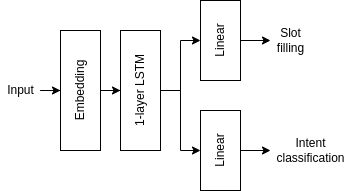
\includegraphics[width=0.8\linewidth]{images/baseline.png}
    \caption{Baseline model.}
    \label{fig:baseline-model}
\end{figure}

\subsection{Model A - Bi-LSTM}
The Model A is an evolution of the baseline model, by using bilinear LSTM. In this case the architecture is slightly more complex:
\begin{itemize}
    \item embedding layer (size 600);
    \item 2-layer bilinear LSTM (size 400). Instead of using only the past, with Bi-LSTM the model can exploit both past and future words at the same time. Such subsequent layers also improve the results;
    \item two heads, one for each one of the two tasks:
    \begin{itemize}
        \item LayerNorm \cite{https://doi.org/10.48550/arxiv.1607.06450}, which is nowadays the standard normalization layer for recurrent-based models \cite{DBLP:journals/corr/VaswaniSPUJGKP17};
        \item Linear.
    \end{itemize}
\end{itemize}

\begin{figure}[!h]
    \centering
    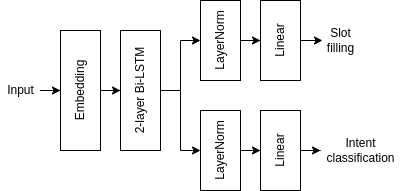
\includegraphics[width=0.8\linewidth]{images/model-a.png}
    \caption{Model A.}
    \label{fig:model-a}
\end{figure}

With this second model, some improvements have been introduced in the training procedure:
\begin{itemize}
    \item As already described, especially the ATIS dataset is very unbalanced. To improve the results, the cross entropy loss is weighted according to the label frequency, so that also less frequent classes can get more importance. For each class $c$:
    \begin{equation*}
        w_c = 1 - \frac{freq_c}{\textrm{dataset size}}
    \end{equation*}
    \item An improved early stopper which takes into account also the loss on the intent classification task.
\end{itemize}

\subsection{Model B - Bi-GRU}
The Model B is a slight modification of the Model A: the main difference is that it uses a bidirectional GRU layer instead of the LSTM one. Even though in terms of performance GRU and LSTM should be similar, the former is more efficient and lightweight. \Cref{fig:model-b} shows Model B's architecture.

\begin{figure}[!h]
    \centering
    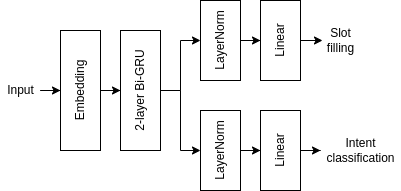
\includegraphics[width=0.8\linewidth]{images/model-b.png}
    \caption{Model B.}
    \label{fig:model-b}
\end{figure}
 

\section{Evaluation}
% \begin{itemize}
%     \item \textit{The metrics you used}
%     \item \textit{Results on evaluation that you performed}
%     \item \textit{Comparison and differences between your model and the baseline}
%     \item \textit{Correct interpretation of errors and analysis}
% \end{itemize}
% (approx. 400-800 words)

\subsection{Metrics}
Following the project instructions, the main two metrics that have been considered are \emph{accuracy} and \emph{F1} score:
\begin{itemize}
    \item Accuracy is an evaluation metric defined as the ratio of true positives and true negatives to all the observations. This value express how likely we can expect a correct prediction from the model. It can be formalized as follows:
    \begin{equation*}
        \textrm{acc} = \frac{TP + TN}{TP + TN + FP + FN}
    \end{equation*}
    where TP, TN, FP, and FN are respectively true positives, true negative, false positives, and false negatives.
    \item F1 score is an evaluation metric that is built on top of precision and recall. This single-value metric is useful when trying to optimize for both precision (very likely that positive predictions are actually positives) and recall (find all the positive cases). It can be formalized as follows:
    \begin{equation*}
        \textrm{f1} = 2 * \frac{precision * recall}{precision + recall}
    \end{equation*}
\end{itemize}

\subsection{Model Scores}
\Cref{tab:model-score} collect the scores of the three proposed models on both the ATIS and SNIPS dataset. Even though these results are far away from the state-of-the-art (achieve with pretrained models, such as BERT \cite{DBLP:journals/corr/abs-1810-04805}, GPT2 \cite{Radford2019LanguageMA}, T5 \cite{DBLP:journals/corr/abs-1910-10683}), Model A and B are able to obtain pretty competitive scores.

\begin{table*}[!t]
    \centering
    \begin{tabular}{lrrrr}
        \toprule
            & \multicolumn{2}{c}{ATIS} & \multicolumn{2}{c}{SNIPS} \\
            Model & Slot F1  & Intent Acc. & Slot F1 & Intent Acc.\\
        \midrule
            Baseline & $0.918 \pm 0.003$ & $0.937 \pm 0.004$ & $0.803 \pm 0.012$ & $0.961 \pm 0.005$ \vspace{0.2cm}\\
            Model A & $\mathbf{0.947 \pm 0.001}$ & $0.965 \pm 0.002$ & $0.899 \pm 0.006$ & $0.971 \pm 0.002$ \vspace{0.2cm}\\
            Model B & $0.946 \pm 0.001$ & $\mathbf{0.968 \pm 0.003}$ & $\mathbf{0.906 \pm 0.006}$ & $\mathbf{0.972 \pm 0.004}$ \\
        \bottomrule
    \end{tabular}
    \caption{Model Scores.}
    \label{tab:model-score}
\end{table*}

\subsection{Results and Interpretation}
Even though the scores seem to be quite decent also for the baseline model, it struggles a lot when dealing with classes that are not frequent: this conclusion is more evident on the ATIS dataset, since it is more unbalanced that SNIPS. In this situation the model tends to overpredict the most common labels, such as \texttt{flight} for intent classification on the ATIS dataset. On the contrary, as provided in \cref{tab:model-score}, the baseline model is already able to obtain good results when dealing with the balanced intent classification task on the SNIPS dataset. 

Moreover, the baseline model struggles when doing slot filling on the ATIS dataset when dealing with numbers departure and arrival information. Even though the model is able to understand if it is dealing with a city, day name, or month number, it is not very good at identifying if it is an information linked to departure or arrival. This problem seems to be partially solved with model A.

Another similar issue that all the models present is the fact they struggle to distinguish between song and album names in the SNIPS dataset.

With respect to the baseline, the model A improves performances of $\sim$2.5\% for both the datasets. Once noticeable improvement is in terms of faster convergence thanks to the higher learning rate. This helps to avoid local minimum and to reduce of the required number of epochs to 1/4 with respect to the baseline.

Even though the performance improvement is not that noticeable, the normalization layer on the model A gives more stability (less variance in model performance) and better gradient flow during the back-propagation of the computational graph.

Further tests have been attempted on model A to increase the number of LSTM layers or the depth of the heads. Even though incrementing the number of parameters is generally a rule of thumb in machine learning, in this case the datasets, especially ATIS, are not big enough: during the training process the model suffered from overfitting. Still, the big improvement on SNIPS (which is bigger than ATIS) of model A with respect to the baseline is probably due to the increment of trainable parameters. Dropout has been tested on model A's heads, but it does not improve the performance.

Finally, Model B obtains very similar accuracies and F1 scores with respect to Model A. As already explained, GRU should guarantee the same performance of LSTM, but with less computational power required, thanks to their simplified cell structure. Specifically, Model B's training is $\sim$10\% faster than Model A's one.

\section{Conclusion}
This work presents and compares three different models by using the ATIS and SNIPS datasets to solve jointly intent classification and slot filling. Moreover, an extensive analysis on results and performance has been carried out, specifically on the dataset composition and model limitations.

Further improvements could be focusing on pretrained models to obtain state-of-the-art results, such as BERT \cite{DBLP:journals/corr/abs-1810-04805}, GPT2 \cite{Radford2019LanguageMA}, and T5 \cite{DBLP:journals/corr/abs-1910-10683}: in this case tokenization and loss computation should be handled carefully. Moreover, to improve the performance on slot filling, also Conditional Random Field (CRF) could be applied \cite{DBLP:journals/corr/HuangXY15}.

\bibliographystyle{IEEEtran}
\bibliography{mybib.bib}

\end{document}